\section{Testaufbau und Szenario}
Die Usability-Tests wurden anhand des Szenarios \emph{Hospital Planning} durchgeführt. 
Die Testpersonen sollten in einem simulierten Planungsmeeting die Position eines Tisches in \textbf{BEDROOM3} vorschlagen, Änderungen nach Feedback der Architekt:in umsetzen und abschliessend den Plan speichern.

\textbf{Aufgabenabfolge:}
\begin{enumerate}
    \item Zwei Minuten freies Zeichnen
    \item Zeichnung komplett löschen
    \item PDF mit Grundriss (\texttt{Hospital\_Floor\_Plan.pdf}) hochladen
    \item Stiftfarbe auf Rot ändern
    \item Tisch links vom Bett in BEDROOM3 einzeichnen
    \item Nach Feedback: Tisch löschen und rechts vom Bett platzieren
    \item Tischmasse 1\,m $\times$ 1\,m skizzieren und Beschriftung \enquote{table} in den Tisch einfügen(nicht massstabsgetreu erforderlich)
    \item Plan lokal speichern
\end{enumerate}

\begin{center}
    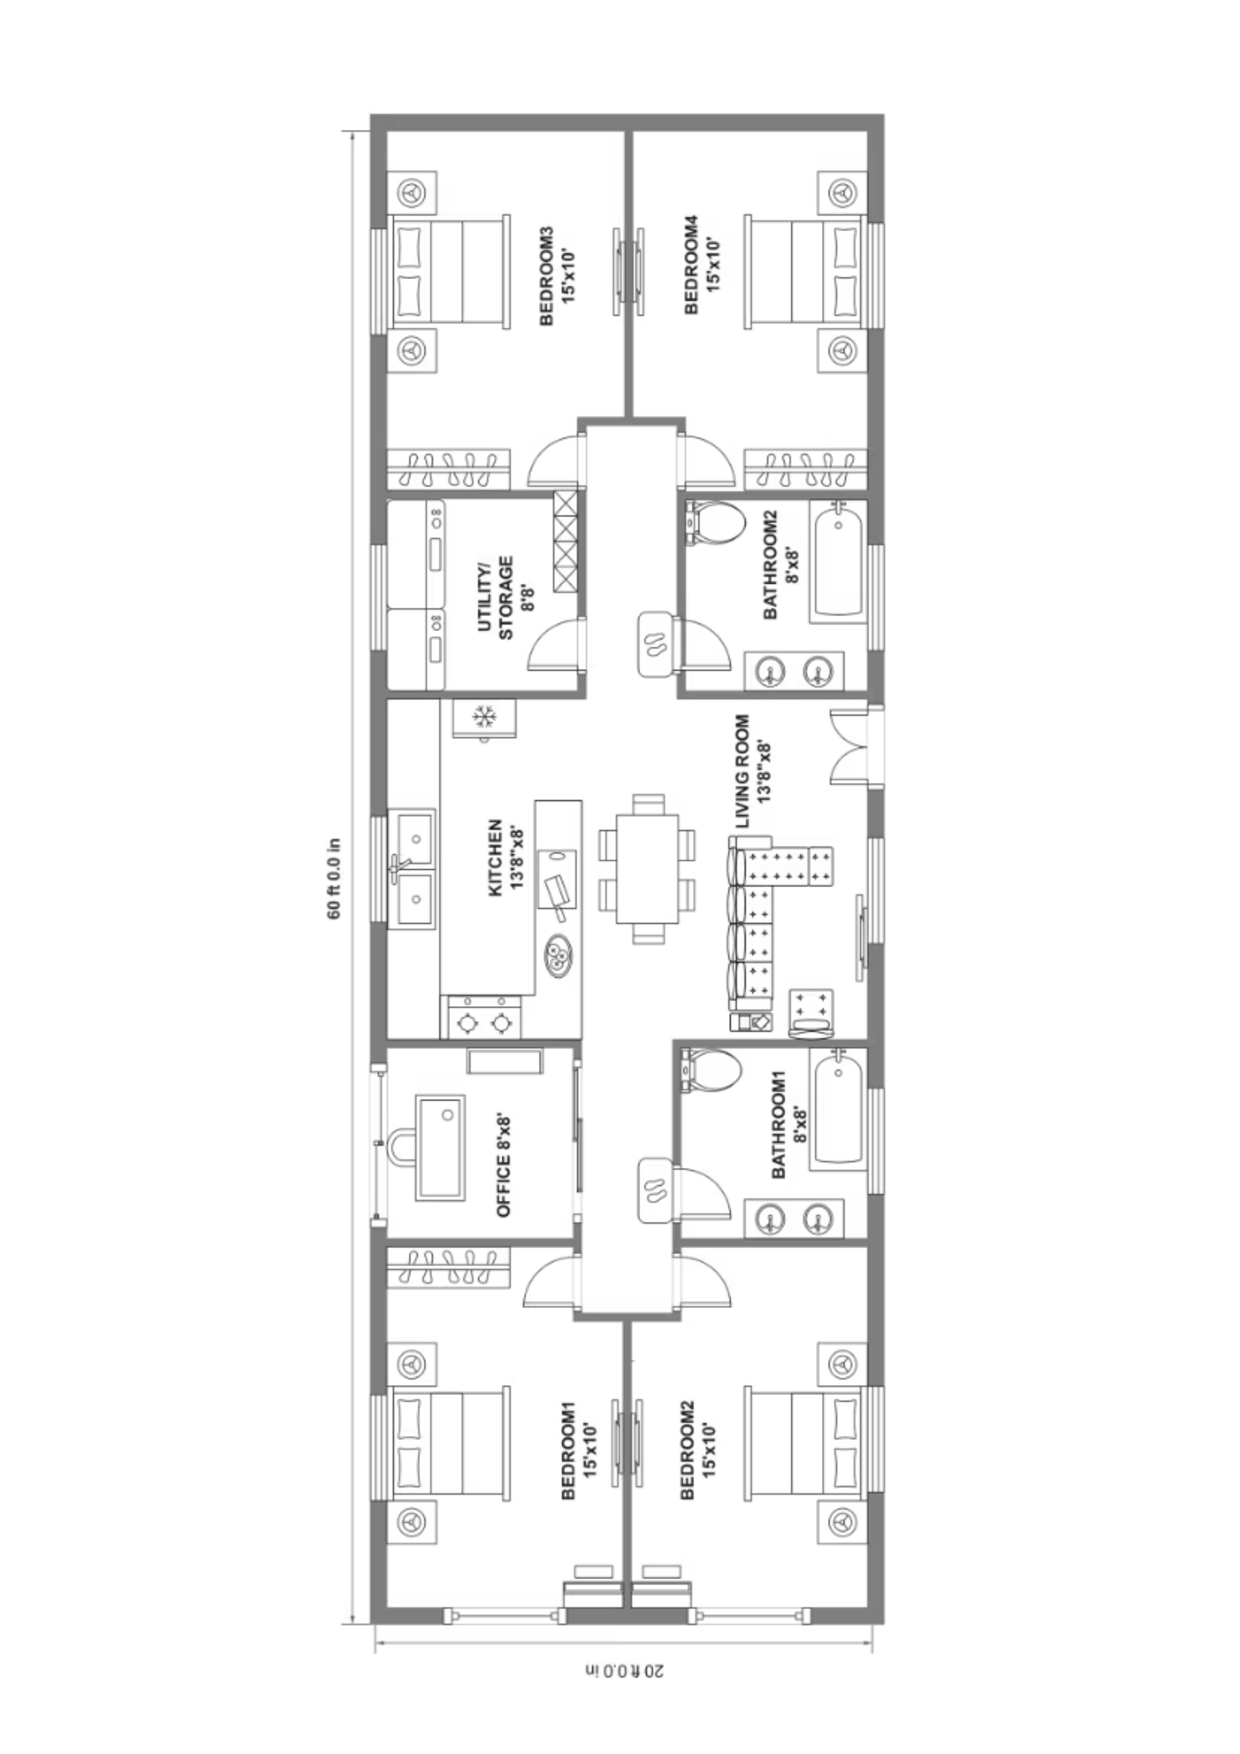
\includegraphics[width=0.65\textwidth]{graphics/Hospital_Floor_Plan.pdf}
    \captionof{figure}{Verwendeter Grundrissplan \texttt{Hospital\_Floor\_Plan.pdf}}
\end{center}
\clearpage

\textbf{SUS-Fragebogen:}  
Nach Abschluss der Aufgaben wurde jeder Testperson der standardisierte \emph{System Usability Scale} (SUS) Fragebogen vorgelegt.

\begin{center}
    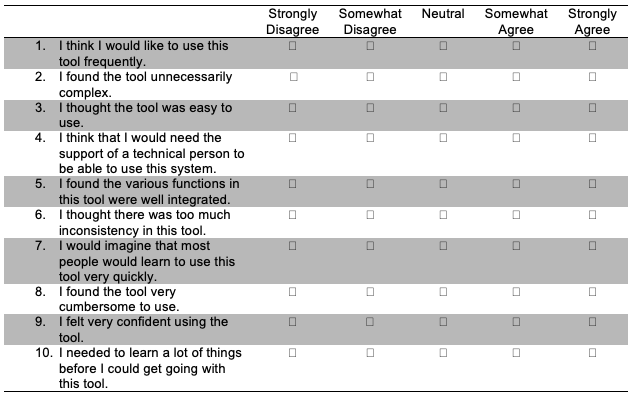
\includegraphics[width=0.95\textwidth]{graphics/sus_blank.png}
    \captionof{figure}{Leerer SUS-Fragebogen (10 Aussagen, 5-stufige Skala von \enquote{Strongly Disagree} bis \enquote{Strongly Agree})}
\end{center}

\textbf{Follow-up-Fragen:}  
Nach der SUS-Bewertung wurden zusätzlich folgende offenen Fragen gestellt:
\begin{enumerate}
    \item \textbf{Was hat Ihnen am Tool am besten gefallen?}
    \item \textbf{Gab es etwas, das verwirrend oder schwierig zu bedienen war?}
    \item \textbf{Fehlt etwas, das Sie erwartet oder gerne gehabt hätten?}
    \item \textbf{Haben Sie Vorschläge, wie das Tool verbessert werden könnte?}
\end{enumerate}
